\chapter{文件管理}\label{OS04}

\section{文件、目录项与索引节点}\label{OS04-objects}

文件是具有名称和属性的持久数据集合。FCB 保存类型、大小、所有者、权限、时间、存储位置等管理信息；采用 inode 时，文件名与其余属性分开，目录项建立名字到 inode 号的关联。inode 号仅在所属文件系统内解释。

\par\smallskip
{\fontsize{9.3}{12}\selectfont\setlength{\tabcolsep}{2.5pt}\setlength{\LTleft}{0pt}\setlength{\LTright}{0pt}
\begin{longtable}{@{}>{\raggedright\arraybackslash}p{\dimexpr0.35030\linewidth-2\tabcolsep\relax}>{\raggedright\arraybackslash}p{\dimexpr0.64970\linewidth-2\tabcolsep\relax}@{}}
\toprule
对象 & 内容与作用 \\

\midrule\endfirsthead\toprule
对象 & 内容与作用 \\

\midrule\endhead\bottomrule\endfoot
目录项 & 文件名、inode 号；目录本身也是文件 \\

磁盘 inode & 文件属性、硬链接计数、块定位等持久信息 \\

内存 inode & 已载入属性及运行时锁、引用状态等 \\

打开实例 & 一次打开的访问方式、当前偏移及 inode 引用 \\

进程描述符表 & 在本进程内把 fd 关联到打开实例 \\

\end{longtable}}
\par\smallskip

知道名字、知道 inode 号、inode 已缓存、数据已缓存分别消除不同访问步骤。教材若把打开实例和内存 inode 合称系统打开表，应先确定字段归属再判断共享关系。

\section{建立、打开、读写、关闭与删除}\label{OS04-operations}

\par\smallskip
{\fontsize{9.3}{12}\selectfont\setlength{\tabcolsep}{2.5pt}\setlength{\LTleft}{0pt}\setlength{\LTright}{0pt}
\begin{longtable}{@{}>{\raggedright\arraybackslash}p{\dimexpr0.28142\linewidth-2\tabcolsep\relax}>{\raggedright\arraybackslash}p{\dimexpr0.71858\linewidth-2\tabcolsep\relax}@{}}
\toprule
操作 & 主要变化 \\

\midrule\endfirsthead\toprule
操作 & 主要变化 \\

\midrule\endhead\bottomrule\endfoot
建立 & 分配控制信息，父目录新增名字；空文件可暂不占数据块 \\

打开 & 路径查找、权限检查、建立或引用打开状态，返回 fd \\

读取 & 按当前偏移定位块，必要时 I/O，复制实际字节并更新位置 \\

写入 & 可分配新块、改变长度、标记缓存为脏，按规则写回 \\

关闭 & 释放本次打开引用，必要时更新元数据 \\

删除名字 & 取消目录关联，减少硬链接数，满足回收条件后释放内容 \\

\end{longtable}}
\par\smallskip

打开无需读入整个文件，写返回成功不必表示已持久化。短读、文件结束、缓存命中及错误按接口和题设。

\par\medskip\Needspace{4\baselineskip}\noindent\hypertarget{OS04-E01}{}\label{OS04-E01}\textbf{例 4-1}\par\nobreak\smallskip

若文件 F 仅被进程 P 打开并访问，则当进程 P 关闭 F 时，文件系统需要完成的是（　）。

A. 删除目录文件中 F 的目录项

B. 释放 F 的索引节点所占的内存空间

C. 释放 F 的索引节点所占的外存空间

D. 将文件磁盘索引节点中的链接计数减 1

两个进程分别 \texttt{open} 同一文件通常各有打开实例与独立偏移，指向共同 inode；\texttt{dup} 或继承共享同一打开实例时可共享偏移。把各进程偏移放在进程打开表、共享属性放在系统表的教材模型，按其字段使用。打开计数与硬链接数分别统计运行引用和名字。单次写的原子性无须推出``读---改---写''事务整体原子，应用仍可能需要锁。

\section{文件保护}\label{OS04-protection}

访问矩阵按主体为行、对象为列，单元格为允许操作集合；按对象列保存为 ACL，按主体行组织为能力表。检查须同时确定身份、所属组、对象和相应操作。

\par\smallskip
{\fontsize{9.3}{12}\selectfont\setlength{\tabcolsep}{2.5pt}\setlength{\LTleft}{0pt}\setlength{\LTright}{0pt}
\begin{longtable}{@{}>{\raggedright\arraybackslash}p{\dimexpr0.29430\linewidth-2\tabcolsep\relax}>{\raggedright\arraybackslash}p{\dimexpr0.70570\linewidth-2\tabcolsep\relax}@{}}
\toprule
方法 & 直接作用及边界 \\

\midrule\endfirsthead\toprule
方法 & 直接作用及边界 \\

\midrule\endhead\bottomrule\endfoot
口令 & 验证访问凭证；保存验证信息，注意凭证泄露与共享 \\

加密 & 用密钥控制内容可读性，算法与密钥管理决定效果 \\

权限表 & 规定主体可执行的读、写、执行等操作，访问时检查 \\

\end{longtable}}
\par\smallskip

每类主体每个独立权限需一位，\(u\) 类、\(r\) 种独立权限需 \(ur\) 位。权限间逻辑蕴含关系须由题设给出。目录查找、列出、修改权限与文件数据权限分开检查。Windows 访问控制中，拒绝条目可影响有效权限；实际合并与继承按系统规则。

\par\medskip\Needspace{4\baselineskip}\noindent\hypertarget{OS04-E02}{}\label{OS04-E02}\textbf{例 4-2}\par\nobreak\smallskip

某文件系统针对每个文件，把用户分成安全管理员、文件主、文件主的伙伴、其他用户 4 类；访问权限有完全控制、执行、修改、读取、写入 5 种。若 FCB 中用二进制位串表示不同类别用户对一个文件的访问权限，至少需要多少位？

A. 5　　B. 9　　C. 12　　D. 20

\section{逻辑结构与记录索引}\label{OS04-records}

无结构文件向应用提供字节序列，应用解释记录边界；有结构文件由定长或变长记录组成。

\par\smallskip
{\fontsize{9.3}{12}\selectfont\setlength{\tabcolsep}{2.5pt}\setlength{\LTleft}{0pt}\setlength{\LTright}{0pt}
\begin{longtable}{@{}>{\raggedright\arraybackslash}p{\dimexpr0.36603\linewidth-2\tabcolsep\relax}>{\raggedright\arraybackslash}p{\dimexpr0.63397\linewidth-2\tabcolsep\relax}@{}}
\toprule
记录组织 & 定位方式及限制 \\

\midrule\endfirsthead\toprule
记录组织 & 定位方式及限制 \\

\midrule\endhead\bottomrule\endfoot
串结构顺序文件 & 按存入先后排列，关键字一般顺序查找 \\

顺序结构顺序文件 & 按关键字有序；适当连续布局下可用有序检索 \\

索引文件 & 索引项保存关键字、记录逻辑地址等，可定位变长记录 \\

索引顺序文件 & 每组一索引，先定位组再组内查找，平衡空间与查找 \\

\end{longtable}}
\par\smallskip

定长、逻辑连续记录，首址 \(F\)、记录长 \(L\)，第 \(i\) 条从0编号时起址 \(F+iL\)；变长须累加长度或另建索引。记录号直接定位、关键字查找分别处理；链接组织仍可能要追链。

\(N\) 条记录分 \(g\) 组，两层均线性扫描且成功位置近似均匀时，平均比较约 \(g/2+N/(2g)\)，\(g\approx\sqrt N\) 时两项平衡；精确成功扫描平均数用各层 \((n+1)/2\)。改用折半或树索引须重算。

用户记录索引映射“关键字\ensuremath{\to}文件内逻辑位置”，系统块分配映射“逻辑块号\ensuremath{\to}物理块号”。每记录 \(L\) B、块 \(B\) B 且 \(B/L\) 为整数、记录不跨块时，第 \(i\) 条的逻辑块为 \(\lfloor iL/B\rfloor\)，块内偏移 \(iL\bmod B\)。逻辑记录结构可搭配不同物理分配方式。

\section{连续、链接与索引分配}\label{OS04-allocation}

下表从文件控制信息已在内存、相关数据和索引尚未缓存出发，访问从0编号的逻辑块 \(k\)。

\par\smallskip
\begin{wideblock}
{\fontsize{9.3}{12}\selectfont\setlength{\tabcolsep}{2.5pt}\setlength{\LTleft}{0pt}\setlength{\LTright}{0pt}
\begin{longtable}{@{}>{\raggedright\arraybackslash}p{\dimexpr0.20982\linewidth-2\tabcolsep\relax}>{\raggedright\arraybackslash}p{\dimexpr0.38208\linewidth-2\tabcolsep\relax}>{\raggedright\arraybackslash}p{\dimexpr0.40810\linewidth-2\tabcolsep\relax}@{}}
\toprule
方式 & 定位与访盘数 & 增长及开销 \\

\midrule\endfirsthead\toprule
方式 & 定位与访盘数 & 增长及开销 \\

\midrule\endhead\bottomrule\endfoot
连续 & 起始块号加 \(k\)，读数据1次 & 顺序、随机方便；扩展受邻接空间限制，有外部碎片 \\

隐式链接 & 从首块沿数据块后继追链，共 \(k+1\) 次读 & 离散追加，指针占数据块空间，不便随机访问 \\

FAT 显式链接 & 内存 FAT 追链后读目标1次 & 全卷表占内存；定位仍可有多次内存追链 \\

索引 & 按块号逐级查索引，经 \(h\) 级间接则 \(h+1\) 次读 & 离散增长，索引块另占空间 \\

\end{longtable}}
\end{wideblock}
\par\smallskip

链接、索引消除整体连续要求，最后一块仍可有内部未用空间。FAT 驻留条件只免除表的访盘。多个索引块可链接，也可用多层索引；链接索引块时查后块仍需追前面的索引块。

\section{混合索引容量与访问路径}\label{OS04-mixed-index}

块 \(B\) B，块号 \(e\) B，每索引块扇出 \(q=\lfloor B/e\rfloor\)。inode 有 \(d\) 个直接项和一级、二级、三级间接项各一个，则理论用户数据长度

\[L_{\max}=(d+q+q^2+q^3)B.\]

须同时满足地址字段、文件大小字段及卷容量等限制；用户长度不含索引块。直接区逻辑块为 \([0,d)\)，一级为 \([d,d+q)\)，二级随后 \(q^2\) 块，三级再后 \(q^3\) 块。

对二级区的逻辑块 \(k\)，先减 \(d+q\) 得区内序号 \(u\)，两层索引依次为 \(\lfloor u/q\rfloor\)、\(u\bmod q\)。读数据前须计未缓存索引块；仅求块号时不加入最终数据块读盘。

\par\medskip\Needspace{4\baselineskip}\noindent\hypertarget{OS04-E03}{}\label{OS04-E03}\textbf{例 4-3}\par\nobreak\smallskip

文件索引节点中有 10 个直接索引指针，一级和二级索引指针各 1 个。磁盘块为 1 KB，每个索引指针 4 B。某文件索引节点已在内存，把该文件偏移量为 1234 和 307400（按字节编址）处所在的磁盘块读入内存，需要访问的磁盘块个数分别是（　）。

A. 1、2　　B. 1、3　　C. 2、3　　D. 2、4

\par\medskip\Needspace{4\baselineskip}\noindent\hypertarget{OS04-E04}{}\label{OS04-E04}\textbf{例 4-4}\par\nobreak\smallskip

一个记录文件采用隐式链接分配，定长逻辑记录为 100 B，采用记录成组分解，盘块为 512 B。目录项已读入内存，对第 22 个逻辑记录完成修改，共启动磁盘多少次？

A. 3　　B. 4　　C. 5　　D. 6

\section{目录结构与路径解析}\label{OS04-directory}

单级目录命名冲突多；两级按用户分目录；树形支持多层分类；无环图允许多个目录关联同一对象，通常限制目录硬链接以避免环。共享目录边与独立复制分别管理生命周期。

绝对路径从根解析，相对路径从当前目录解析；\texttt{.\allowbreak{}} 为本目录，\texttt{.\allowbreak{}.\allowbreak{}} 为父目录。每个分量通过目录项找到下级 inode，再查下级目录；实际 I/O 由各层目录、inode 与数据缓存决定。当前目录可省去共同前缀查找，权限检查继续执行。

分离文件名与 inode 可缩小目录项。块 \(B\) B、目录项 \(e\) B、项不得跨块时，每块容纳 \(\lfloor B/e\rfloor\) 项。若共 \(b\) 个满目录块、目标均匀分布且逐块成功查找，平均读 \((b+1)/2\) 个目录块；再按缓存补计 inode 读取。哈希、树索引或末块不满时按实际概率计算。

\section{硬链接、符号链接与回收}\label{OS04-links}

\par\smallskip
\begin{wideblock}
{\fontsize{9.3}{12}\selectfont\setlength{\tabcolsep}{2.5pt}\setlength{\LTleft}{0pt}\setlength{\LTright}{0pt}
\begin{longtable}{@{}>{\raggedright\arraybackslash}p{\dimexpr0.20914\linewidth-2\tabcolsep\relax}>{\raggedright\arraybackslash}p{\dimexpr0.42861\linewidth-2\tabcolsep\relax}>{\raggedright\arraybackslash}p{\dimexpr0.36224\linewidth-2\tabcolsep\relax}@{}}
\toprule
项目 & 硬链接 & 软／符号链接 \\

\midrule\endfirsthead\toprule
项目 & 硬链接 & 软／符号链接 \\

\midrule\endhead\bottomrule\endfoot
保存关系 & 目录项直接指向同一 inode & 独立链接文件保存目标路径 \\

目标计数 & 增删名字改变目标硬链接数 & 不因此增加目标硬链接数 \\

跨文件系统 & 通常受限 & 可跨文件系统 \\

目录与失效 & 通常限制任意目录硬链接；删除一个名其余可用 & 可指目录；保存路径消失后可悬空 \\

\end{longtable}}
\end{wideblock}
\par\smallskip

目标硬链接数归零且无有效使用引用等条件满足后才回收数据和 inode；已打开但无名字的文件可继续使用至相应引用释放。符号链接相对目标通常相对于链接所在目录解释。两个硬链接共享文件身份，独立打开仍可有独立位置。

\begin{figure}
\centering
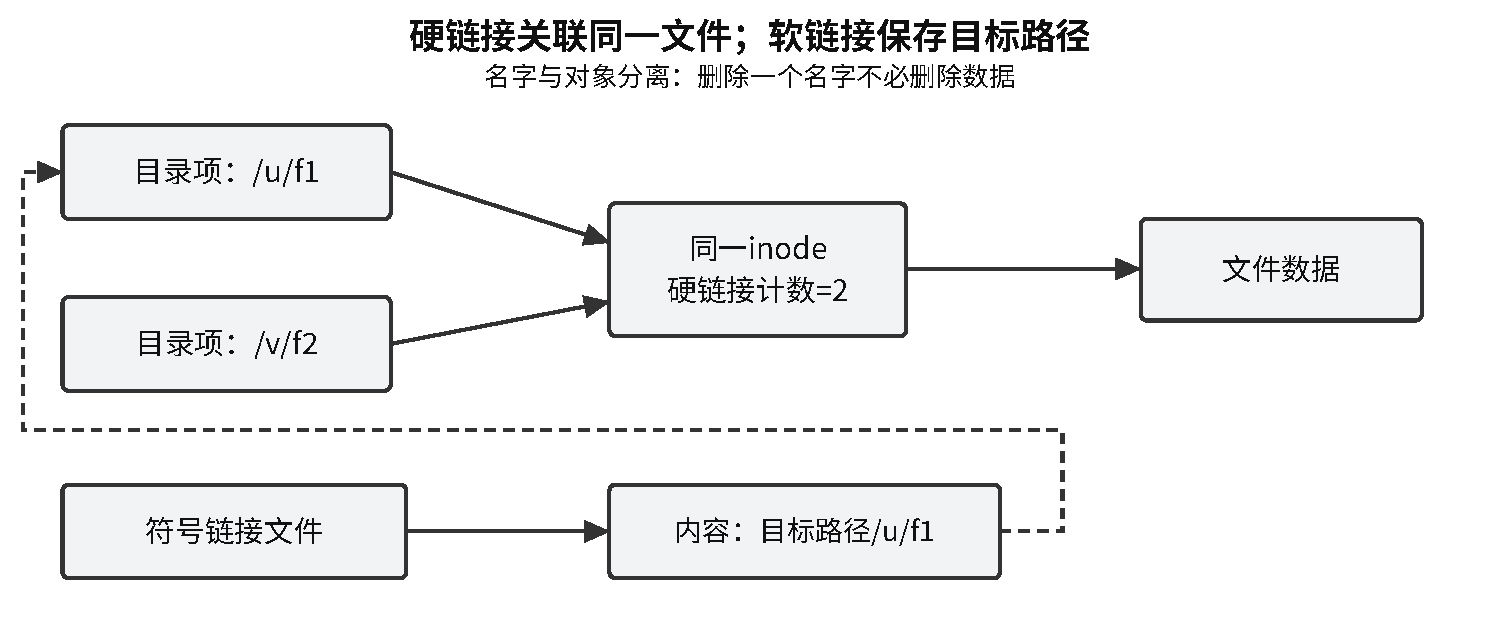
\includegraphics[width=\linewidth,height=108mm,keepaspectratio]{figures/OS_file_links.pdf}
\caption{名字、inode 与目标路径的不同关系}
\end{figure}

\par\medskip\Needspace{4\baselineskip}\noindent\hypertarget{OS04-E05}{}\label{OS04-E05}\textbf{例 4-5}\par\nobreak\smallskip

若文件 f1 的硬链接为 f2，两个进程分别打开 f1、f2，获得文件描述符 fd1、fd2，则正确的是（　）。

Ⅰ. f1 和 f2 的读写指针位置保持相同

Ⅱ. f1 和 f2 共享同一个内存索引节点

Ⅲ. fd1 和 fd2 分别指向各自的用户打开文件表中的一项

A. 仅Ⅲ　　B. 仅Ⅱ、Ⅲ　　C. 仅Ⅰ、Ⅱ　　D. Ⅰ、Ⅱ、Ⅲ

\section{文件系统分层与持久结构}\label{OS04-fs-structures}

\par\smallskip
{\fontsize{9.3}{12}\selectfont\setlength{\tabcolsep}{2.5pt}\setlength{\LTleft}{0pt}\setlength{\LTright}{0pt}
\begin{longtable}{@{}>{\raggedright\arraybackslash}p{\dimexpr0.41421\linewidth-2\tabcolsep\relax}>{\raggedright\arraybackslash}p{\dimexpr0.58579\linewidth-2\tabcolsep\relax}@{}}
\toprule
职责 & 典型工作 \\

\midrule\endfirsthead\toprule
职责 & 典型工作 \\

\midrule\endhead\bottomrule\endfoot
用户接口与目录系统 & 接收系统调用、路径查找、管理打开关系 \\

存取控制 & 检查主体权限 \\

逻辑文件系统 & 记录号转换为文件内逻辑位置 \\

物理文件系统 & 逻辑块到设备块位置 \\

辅助分配 & 空间分配回收 \\

设备管理 & 缓冲、I/O 调度、启动及完成处理 \\

\end{longtable}}
\par\smallskip

层名可按教材模型合并，责任对应关系保持清楚。删除末尾记录时，仍含保留数据的末块须保留，只更新长度等相关信息。

磁盘引导信息服务启动，卷控制块／超级块记录块长、规模、空闲管理等；目录、inode 区记录文件及名字，数据区保存内容。MBR 属整盘引导和分区管理，卷内引导块属于相应卷，布局采用题设。

内存维护挂载信息、目录与 inode 缓存、打开对象和进程描述符表。扩展文件可同时改变位图、inode、数据与索引，部分写入后崩溃可能不一致；一致性检查按引用与分配关系核对，日志按提交和重放规则恢复，保证范围由记录对象与写回规则决定。

\section{空闲空间管理与位图}\label{OS04-free-space}

\par\smallskip
{\fontsize{9.3}{12}\selectfont\setlength{\tabcolsep}{2.5pt}\setlength{\LTleft}{0pt}\setlength{\LTright}{0pt}
\begin{longtable}{@{}>{\raggedright\arraybackslash}p{\dimexpr0.30259\linewidth-2\tabcolsep\relax}>{\raggedright\arraybackslash}p{\dimexpr0.69741\linewidth-2\tabcolsep\relax}@{}}
\toprule
方法 & 组织与分配回收 \\

\midrule\endfirsthead\toprule
方法 & 组织与分配回收 \\

\midrule\endhead\bottomrule\endfoot
空闲表 & 连续空闲区起点、长度；选区后切分，回收按物理邻接合并 \\

空闲盘块链 & 每块为节点，申请多个块须逐次追链，适合离散分配 \\

空闲盘区链 & 每节点是一段连续区，记录长度与后继，可批量分出 \\

位图 & 每受管块一位，0／1 空闲约定按题设，适合连续或离散分配 \\

成组链接 & 当前组的空闲块号栈及后续组入口，按组装入与保存 \\

\end{longtable}}
\par\smallskip

管理 \(N\) 块，位图需 \(N\) 位，向上取整为 \(\lceil N/8\rceil\) B；大小由管理范围决定。块号与字、位均0基，字长 \(n\) 位时：

\[b=ni+j,\quad i=\lfloor b/n\rfloor,\quad j=b\bmod n.\]

三者均1基时：\(b=n(i-1)+j\)，\(i=\lfloor(b-1)/n\rfloor+1\)，\(j=(b-1)\bmod n+1\)。位图磁盘起始块在算出位图内相对位置后加入。

\par\medskip\Needspace{4\baselineskip}\noindent\hypertarget{OS04-E06}{}\label{OS04-E06}\textbf{例 4-6}\par\nobreak\smallskip

文件系统用位图表示磁盘空间分配，位图存于磁盘 32---127 号块，每块 1024 B，盘块和块内字节都从 0 编号。释放盘块号 409612 时，要修改的位所在盘块号和块内字节序号分别为（　）。

A. 81、1　　B. 81、2　　C. 82、1　　D. 82、2

成组链接在当前组最后的承载块内保存下一组：分配到它时，先读出下一组再交付承载块；回收时组未满则压栈，组已满则把整组写入新回收块，让内存组改为该块入口。终止标记不计作可分配块号，内存与磁盘分配元数据须按规定同步。

\section{VFS 与挂载}\label{OS04-vfs}

VFS 提供统一操作抽象，经操作函数入口分派到具体文件系统；磁盘格式可分别设计。vnode 是内存统一虚拟节点，保存通用信息与操作函数指针；Linux 式抽象进一步区分超级块、inode、dentry、file 对象，分别描述已挂载卷、文件本体、名字关系和一次打开。

挂载将新文件系统根接到现有挂载点；原有下层内容通常被当前视图遮蔽，继续保留。卸载须处理使用引用与待写回信息。具体文件系统须向 VFS 注册所需信息和操作入口。

\section{目录、索引与容量综合}\label{OS04-comprehensive}

名称查找、inode 读取、索引定位、数据读取分别计未缓存成本。文件数量同时受 inode 数、每文件数据块数、间接索引开销及题给其他资源限制，取最紧上界。

\par\medskip\Needspace{4\baselineskip}\noindent\hypertarget{OS04-E07}{}\label{OS04-E07}\textbf{例 4-7}\par\nobreak\smallskip

某文件系统的磁盘块大小为 4 KB，目录项由文件名和索引节点号构成，每个索引节点占 256 字节，其中包含直接地址项 10 个，一级、二级和三级间接地址项各 1 个，每个地址项占 4 字节。该文件系统中子目录 stu 的结构如下图所示，stu 包含子目录 course 和文件 doc，course 子目录包含文件 course1 和 course2。各文件的文件名、索引节点号、占用磁盘块的块号如图中表所示。请回答下列问题。

\begin{figure}
\centering
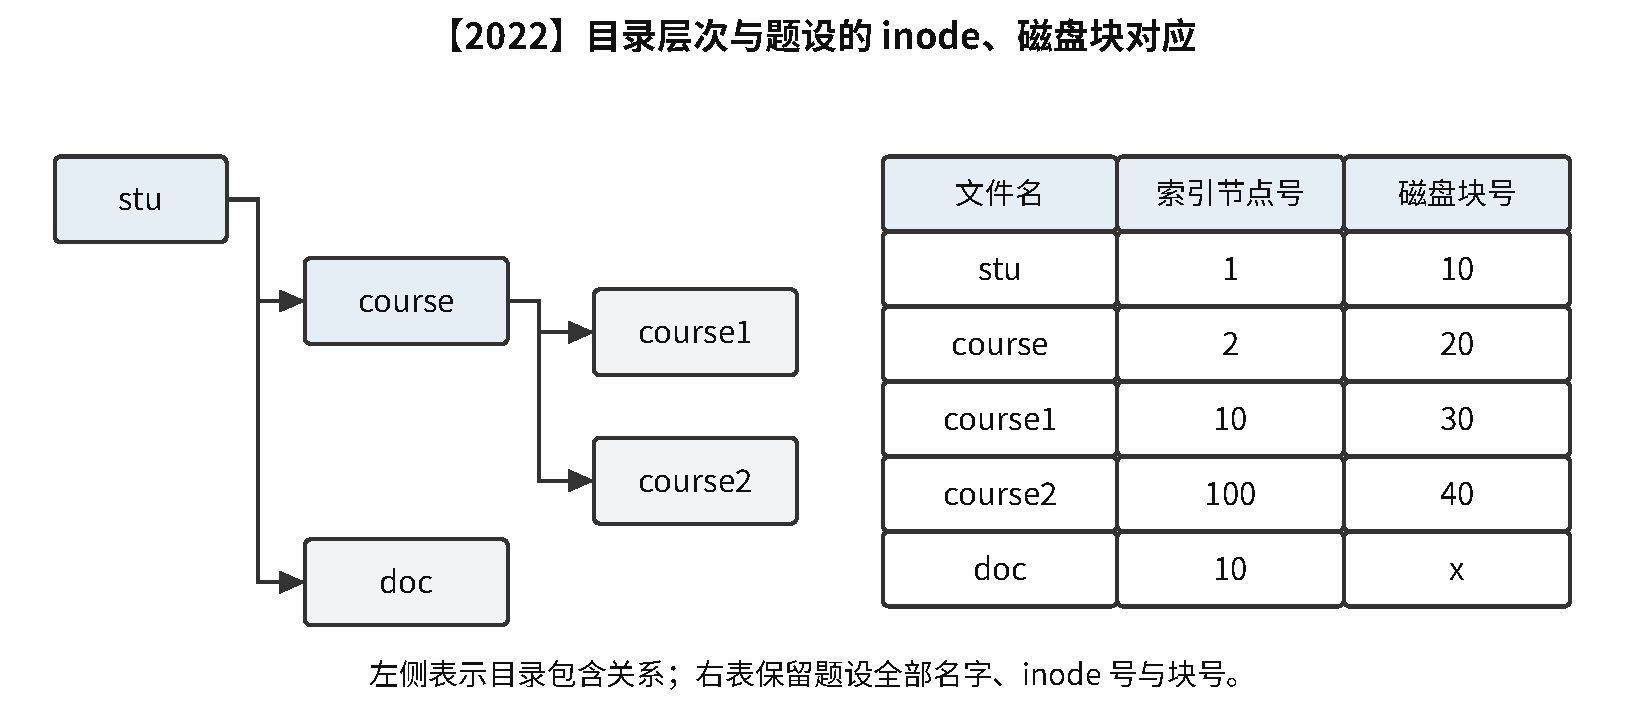
\includegraphics[width=\linewidth,height=108mm,keepaspectratio]{figures/OS_file_directory_2022.pdf}
\caption{stu、course 的目录层次，以及各文件的索引节点号和数据块号}
\end{figure}

（1）目录文件 stu 中每个目录项的内容是什么？

（2）文件 doc 占用的磁盘块的块号 x 的值是多少？

（3）若目录文件 course 的内容已在内存，则打开文件 course1 并将其读入内存，需要读几个磁盘块？说明理由。

（4）若文件 course2 的大小增长到 6 MB，则为了存取 course2 需要使用该文件索引节点的哪几级间接地址项？说明理由。

\par\medskip\Needspace{4\baselineskip}\noindent\hypertarget{OS04-E08}{}\label{OS04-E08}\textbf{例 4-8}\par\nobreak\smallskip

某文件系统采用索引节点存放文件的属性和地址信息，簇大小为 4 KB。每个文件索引节点占 64 B，有 11 个地址项，其中直接地址项 8 个，一级、二级和三级间接地址项各 1 个，每个地址项长度为 4 B。请回答下列问题。

（1）该文件系统能支持的最大文件长度是多少？（给出计算表达式即可。）

（2）文件系统用 1M（\(1\mathrm{M}=2^{20}\)）个簇存放文件索引节点，用 512M 个簇存放文件数据。若一个图像文件的大小为 5600 B，则该文件系统最多能存放多少个这样的图像文件？

（3）若文件 F1 的大小为 6 KB，文件 F2 的大小为 40 KB，则该文件系统获取 F1 和 F2 最后一个簇的簇号需要的时间是否相同？为什么？
